% Suggested insertion for Geometry Before Fields
% Status: cosmology-owned R1 result; no BHSM microscopic normalization claim.
% Recommended placement: after the action-native matter/backreaction section
% and before observable-specific kernels.

\section{Coupled environmental realization of the physical $n=2$ state}
\label{sec:coupled-environmental-state}

The action-native R1 system uses minimally coupled ideal dust and radiation
in the constraint-reduced ADM plus Schutz--Sorkin action audited in
Appendix~\ref{sec:action-native-gradient-dispersion}.
The retained matter--topography system is not restricted to an isolated
two-state topographic evolution.  At the anchor $z_i=2.1$, use the physical
coordinates
\begin{equation}
Y_i=
\left(
q_2,\Pi_2,
\delta_m,\delta_r,v_m,v_r
\right)_i ,
\qquad
q_2=\zeta,
\qquad
\Pi_2=2a^3G_{S,2}\dot\zeta .
\end{equation}
Densities and velocity potentials use the retained ADM convention.
The reference-normalized coordinate $\Pi_2$ need not equal the canonical
$p_\zeta$ of the full coupled action.
The same frozen linear system may be written in block form as
\begin{equation}
\begin{pmatrix}
X_2(z)\\
E(z)
\end{pmatrix}
=
\begin{pmatrix}
U_{XX}(z,z_i) & U_{XE}(z,z_i)\\
U_{EX}(z,z_i) & U_{EE}(z,z_i)
\end{pmatrix}
\begin{pmatrix}
X_2(z_i)\\
E(z_i)
\end{pmatrix},
\end{equation}
where
\begin{equation}
X_2=(q_2,\Pi_2)^T,
\qquad
E=(\delta_m,\delta_r,v_m,v_r)^T .
\end{equation}

An independent reconstruction of the frozen six-state system reproduces the
retained two-column topographic seed within $10^{-12}$ and the stored
full canonical propagator at $z=1.5$ within $10^{-8}$.  Setting the
initial topographic pair to zero and varying the environmental coordinates
alone gives a nonzero $2\times4$ transfer $U_{XE}$. The audit evaluates
linear basis responses; no physical environmental state is inferred or fitted.
Its reproducible implementation is
\texttt{scripts/audit\_r1\_coupled\_environmental\_state.py}.

\begin{table}[htbp]
\centering
\caption{Frozen R1 environmental transfer to $(\zeta,\dot\zeta)$.
The tabulated singular values and matter-subblock determinants use this
output basis, not $(q_2,\Pi_2)$. Their magnitudes depend on coordinate
normalization; rank is unchanged by the invertible output conversion.}
\label{tab:coupled-environment-rank}
\begin{tabular}{cccc}
\toprule
$z$ & $s_1$ & $s_2$ &
$\det\widehat U_{XE}^{(\delta_m,v_m)}$\\
\midrule
1.50 & 9.653252 & 0.00168034 & 0.0162207\\
1.00 & 7.213900 & 0.00988895 & 0.0713376\\
0.50 & 4.138611 & 0.02289428 & 0.0947501\\
0.00 & 3.281912 & 0.01582573 & 0.0519383\\
\bottomrule
\end{tabular}
\end{table}

The two output conventions obey
$U_{XE}=\operatorname{diag}(1,2a^3G_{S,2})\widehat U_{XE}$,
with a positive second diagonal entry on the audited branch.
At all eight sampled post-anchor epochs
$z=1.5,1.0,0.8,0.5,0.3,0.1,0.02,0$,
\begin{equation}
\boxed{\operatorname{rank}U_{XE}=2.}
\end{equation}
Moreover, the matter-only subblock built from $(\delta_m,v_m)$ has nonzero
determinant at these sampled epochs. The environmental block is zero at the
anchor itself; no continuous-interval rank theorem is claimed.  Thus both temporal components of
the later topographic state can be generated by specified environmental
density and velocity data; radiation is not required for temporal full rank.
An isolated one-dimensional temporal attractor is therefore not required
for this coupled realization.

The spatial statement is separate.  The full scalar $n=2$ harmonic sector on
$S^3$ has dimension nine.  On the isotropic R1 background the same temporal
transfer acts independently on each harmonic component.  Writing
\begin{equation}
X(z)\in\mathbb R^{2\times9},
\qquad
E_i\in\mathbb R^{4\times9},
\end{equation}
one has
\begin{equation}
\boxed{
X(z)=U_{XX}(z)X_i+U_{XE}(z)E_i .
}
\end{equation}
The environment can therefore transmit an $n=2$ orientation already present
in its coefficient tensors, but isotropic R1 dynamics do not generate a
preferred axis from an isotropic state.

A one-profile reduction,
\begin{equation}
X(z)=x(z)e^T ,
\end{equation}
requires a common spatial profile across the evolution and, at each epoch,
\begin{equation}
\boxed{
\operatorname{rank}_{\rm spatial}X(z)\le1.
}
\end{equation}
A sufficient condition is $X_i=x_i e^T$ and $E_i=\epsilon_i e^T$, including
$X_i=0$. Environmental alignment alone does not constrain an independently
oriented initial topographic state. A rank-one snapshot does not by itself
establish one fixed profile for the entire history.
Generic multi-pattern environmental data need not satisfy this condition and
can produce spatial rank two.

The resulting prediction problem is therefore not to find an isolated
self-selected topographic eigenline.  It is to specify or derive the physical
environmental state, its full $n=2$ spatial coefficients, and the justified
spatial reduction used by a given observable. The existing reference kernels
and prospective gates retain their declared scope: a generic multi-profile
environment is not silently substituted into single-profile forecasts.

\paragraph{Claim boundary.}
This result begins at the retained R1 anchor $z_i=2.1$.  It does not derive the
anchor state from earlier cosmological initial conditions, does not determine
the absolute microscopic BHSM--R1 normalization, and does not select a unique
global spatial profile or axis.  It establishes only that, once the coupled
environmental state is specified at the anchor, the frozen R1 dynamics allow
that environment to control both temporal components of the later
topographic response without retuning.

Figure~\ref{fig:coupled-environment} displays the sampled transfer diagnostics
in their original output basis.
\begin{figure}[p]
\centering
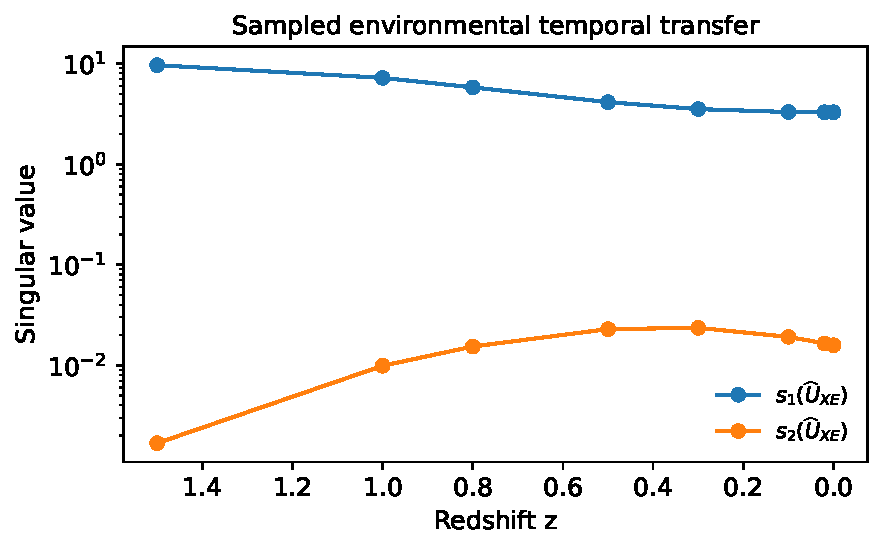
\includegraphics[width=0.82\linewidth]{figures/coupled_environment_singular_values.pdf}\\[0.5em]
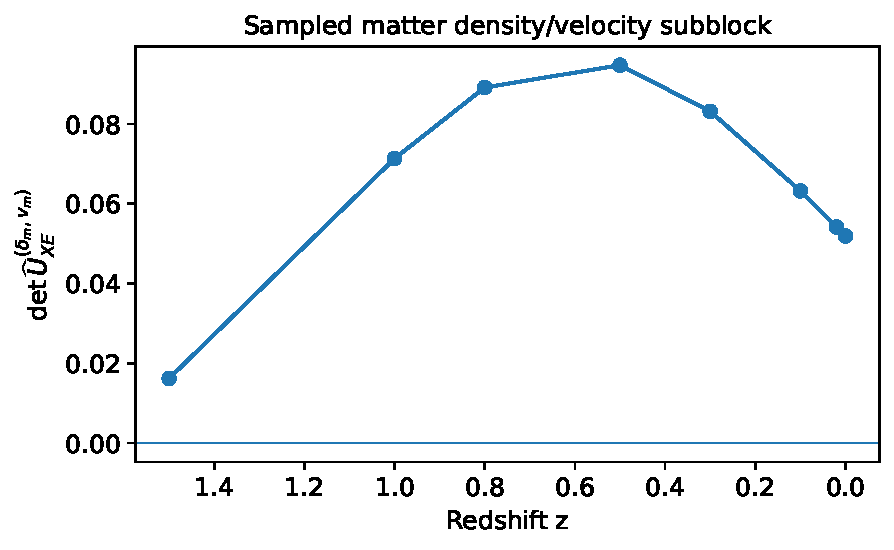
\includegraphics[width=0.82\linewidth]{figures/coupled_environment_matter_determinant.pdf}
\caption{Environmental transfer in the $(\zeta,\dot\zeta)$ output basis: singular values of $\widehat U_{XE}$ (top) and its matter-density/velocity subblock determinant (bottom). Points are the eight audited post-anchor epochs; lines only guide the eye. Both temporal components are accessible there. Singular-value magnitudes depend on coordinate normalization; rank is unchanged by the positive conversion to $(q_2,\Pi_2)$. The block vanishes at the anchor, which is not plotted. This is not spatial profile or axis selection.}
\label{fig:coupled-environment}
\end{figure}
